\documentclass{homework}

\usepackage[nottoc,numbib]{tocbibind}
\usepackage{amsthm}
\usepackage{titlesec}
\usepackage{caption}
\usepackage{wrapfig,lipsum,booktabs}

\usepackage{algorithm2e}
\RestyleAlgo{ruled}
\SetKwComment{Comment}{/* }{ */}

\makeatletter
\renewcommand{\algorithmcfname}{Algoritmo}
\makeatother

\SetKwFor{While}{mientras }{}{fin}
\SetKwFor{For}{para cada }{}{fin}
\SetKwFor{If}{si}{}{fin}
%\SetKwFor{eIf}{si}{}{en otro caso}
% \SetKwFor{For}{para cada:}{}{}
%\SetKwFor{KwData}{Dato:}{}{}
%\SetKwFor{Data}{Dato:}{}{}
\SetKwFor{Results}{resultado}{}{}

\titleclass{\subsubsubsection}{straight}[\subsection]

\newcounter{subsubsubsection}[subsubsection]
\renewcommand\thesubsubsubsection{\thesubsubsection.\arabic{subsubsubsection}}
\renewcommand\theparagraph{\thesubsubsubsection.\arabic{paragraph}} % optional; useful if paragraphs are to be numbered

\titleformat{\subsubsubsection}
  {\normalfont\normalsize\bfseries}{\thesubsubsubsection.}{1em}{}
\titlespacing*{\subsubsubsection}
{0pt}{3.25ex plus 1ex minus .2ex}{1.5ex plus .2ex}

\makeatletter
\renewcommand\paragraph{\@startsection{paragraph}{5}{\z@}%
  {3.25ex \@plus1ex \@minus.2ex}%
  {-1em}%
  {\normalfont\normalsize\bfseries}}
\renewcommand\subparagraph{\@startsection{subparagraph}{6}{\parindent}%
  {3.25ex \@plus1ex \@minus .2ex}%
  {-1em}%
  {\normalfont\normalsize\bfseries}}
\def\toclevel@subsubsubsection{4}
\def\toclevel@paragraph{5}
\def\toclevel@paragraph{6}
\def\l@subsubsubsection{\@dottedtocline{4}{7em}{4em}}
\def\l@paragraph{\@dottedtocline{5}{10em}{5em}}
\def\l@subparagraph{\@dottedtocline{6}{14em}{6em}}
\makeatother

\setcounter{secnumdepth}{4}
\setcounter{tocdepth}{4}


\newtheorem{theorem}{Teorema}[section]
\newtheorem{corollary}{Corolario}[theorem]
\newtheorem{lemma}[theorem]{Lema}
\newtheorem{proposition}[theorem]{Proposición}

\renewcommand{\lstlistingname}{Código}
\captionsetup[table]{name=Tabla}


\title{Práctica 3: Algoritmos Voraces}
\author{Shao Jie Hu Chen \\ Mario Megías Mateo \\ Jesús Samuel García Carballo}
\renewcommand{\course}{Algorítmica}
% \date{1 de abril de 2022}

\begin{document}
    \renewcommand{\refname}{Bibliografía}
    \renewcommand{\contentsname}{Índice de Contenidos}
    \renewcommand{\listtablename}{Lista de Tablas}
    
    \maketitle
    \tableofcontents
    \newpage

    \section{Introducción}
    Un algoritmo greedy es aquel al que se le aplica un enfoque greedy para su resolución, es decir, el que reúne las 6 características siguientes:
\begin{itemize}
    \item Conjunto de candidatos.
    \item Lista de candidatos ya usados.
    \item Un criterio solución, cuando se forma una solución no necesariamente óptima.
    \item Un criterio de factibilidad, candidatos que podrán llegar a ser solución.
    \item Una función de selección que indica el candidato más prometedor de los no usados.
    \item Una función objetivo que a cada solución le asocia un valor, y es la función que intentamos optimizar.
\end{itemize}

Este conjunto de algoritmos no alcanzan soluciones optimales siempre, pueden alcanzar óptimos locales, pero no los globales de los problemas.
Por eso se debe demostrar la corrección del algoritmo.
    \newpage

    \section{Logística de contenedores}
    En este ejercicio dado un buque mercante cuya capacidad de carga es de K toneladas y un conjunto de contenedores $c_1,...,c_n$ cuyos
pesos respectivos son $p_1,...,p_n$, debemos hallar un algoritmo que maximice el número de contenedores cargados y otro que intente 
maximizar el número de toneladas cargadas.

\subsection{Maximización de contenedores}

En primer lugar, debemos ser conscientes de que la capacidad del buque debe ser menor que la suma total de los pesos 
de los contenedores, pues en caso contrario, no estaría bien definido el problema. Para resolver este problema tenemos que darnos cuenta
que lo que nos interesa es ir cogiendo aquellos contenedores cuyo peso sea más pequeño e ir introduciéndolos en el buque mientras que su suma 
sea menor que la capacidad de carga del buque, puesto que el resultado debe tener el mayor número de contenedores posible, sin importar las 
toneladas totales. 

\begin{algorithm}[H]
    \caption{Algoritmo para maximizar el número de contenedores}\label{alg:max_containers}
    \begin{minipage}{0.92\textwidth}
    \textbf{Parámetro}: containers (vector de enteros)

    \textbf{Parámetro}: K (capacidad del buque)

    \end{minipage}

    weight = 0\;
	container = 0\;
    vector result\;
  
    sort(pesos.begin(), pesos.end());

    \While{$weight <= K$ y $container <= containers.size$}{
        result.push\_back(containers.at(container))\;
        weight += containers.at(container)\;
        container++\;
    }
  
    \Return{result}
    
\end{algorithm}

Como vemos en el algoritmo la clave del proceso es antes de añadir los contenedores, ordenarlos de forma creciente para que 
en el ciclo siempre se vaya añadiendo el contenedor con menor peso.

\subsubsection{Condición de optimalidad}
Sea $S = {p_1,...,p_n}$ un conjunto de soluciones para el algoritmo y $S_g = {p_{g_1},...,p_{g_n}}$ las soluciones para el algoritmo Greedy

\subsection{Maximización de toneladas}
En este caso tenemos que maximizar las toneladas por lo que para ello una buena estrategia ir cogiendo osdjavzxnckñn
    \newpage

    \section{Problema del Viajante de Comercio}
    El problema que se nos presenta es, dados $k$ vectores ordenados de menor a mayor,
cada uno con $n$ elementos, combinarlos en un único vector con todos los elementos
ordenados de la misma manera. Al igual que antes, presentamos una solución obvia y
otra empleando un algoritmo Divide y Vencerás. 

\subsection{Caso obvio}

En este caso una alternativa es ir iterando sobre cada vector, añadiendo los elementos
del vector de forma ordenada sobre un acumulador. Ello queda ilustrado en la figura
\ref{fig:2a-obvio}, donde primer se unen los vectores que están en rojo y morado para,
a continuación, unir ese resultado con el vector en verde, dando como resultado
un vector global ordenado. 

\begin{figure}
    \centering
    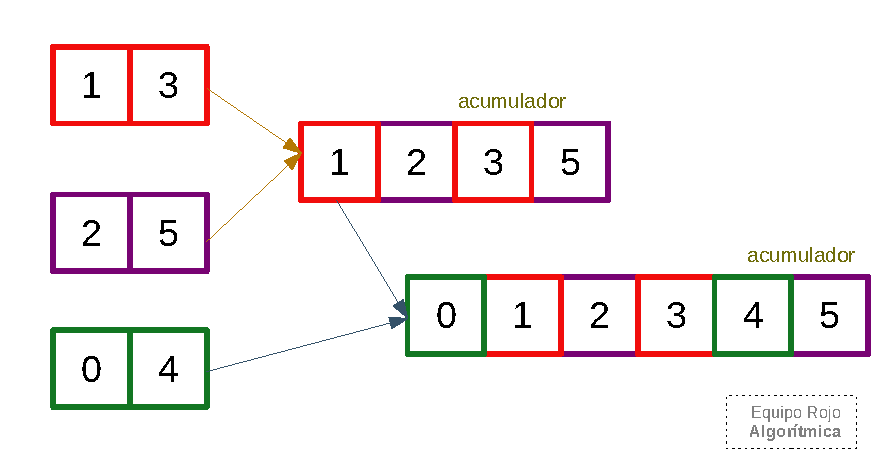
\includegraphics[scale=0.87]{img/orden_2a.pdf}
    \caption{Esquema de funcionamiento del algoritmo de 
    mezcla obvio. Elaboración propia.}
    \label{fig:2a-obvio}
\end{figure}

\subsubsection{Pseudocódigo}

\lstinputlisting[caption=Pseudocódigo asociado a la mezcla 
ordenada de vectores ordenados en el caso obvio., 
label={alg:2a-obvio}]{listing/ejer2a-pseudo-obvio.txt}

\subsubsection{Implementación}

\lstinputlisting[firstline=81, lastline=130, language=C++,
caption=Implementación del algoritmo \ref{alg:2a-obvio}.]{../src/ejercicio-2-mezcla.cpp}

\subsubsection{Análisis de Eficiencia}

En primer lugar, analizamos la \textbf{eficiencia teórica}. En este caso,
el tamaño del problema depende tanto del número de componentes
de los vectores $n$ como del número de vectores $k$ que hemos
considerado. 

Analizando el algoritmo auxiliar UNIFICA de \ref{alg:2a-obvio}, tenemos que el 
número de operaciones que se realiza es independiente
del número de vectores $k$ a considerar, por lo que queda
acotada por una constante. Por su parte, el número de componentes de los
vectores sí influye en el número de operaciones, pues en el ciclo while se recorre completamente
el uno de los vectores y parcialmente la otra, siendo las restantes componentes recorridas
a continuación, por lo que se realizan $cn$ operaciones elementales,
con $c \in \mathbb N$ constante. 

Notemos que el número de operaciones que
se realizan es independiente de los valores de los vectores,
por lo que el mejor caso y el peor caso tienen el mismo orden
de eficiencia. Por tanto, tenemos que su eficiencia es $\theta(n)$. 

% \begin{wraptable}{b}{0.3\linewidth}
\begin{table}
    \footnotesize
    \centering
    \begin{tabular}{|r|r|}
        \hline
        $N$ & $T$ $(\mu s)$ \\
        \hline
        1 & 0.0031 \\ 
        51 & 0.0100 \\ 
        101 & 0.0106 \\ 
        151 & 0.0135 \\ 
        201 & 0.0150 \\ 
        251 & 0.0209 \\ 
        301 & 0.0245 \\ 
        351 & 0.0268 \\ 
        401 & 0.0283 \\ 
        451 & 0.0337 \\ 
        501 & 0.0359 \\ 
        551 & 0.0445 \\ 
        601 & 0.0498 \\ 
        651 & 0.0475 \\ 
        701 & 0.0537 \\ 
        751 & 0.0536 \\ 
        801 & 0.0592 \\ 
        851 & 0.0659 \\ 
        901 & 0.0681 \\ 
        951 & 0.0683 \\ 
        \hline
    \end{tabular}
    \caption{Tiempos de ejecución para el algoritmo \ref{alg:2a-obvio}.}
    \label{tab:2a-obvio-n}
% \end{wraptable}
\end{table}

Para el algoritmo AGRUPA de \ref{alg:2a-obvio}, que es el que nos interesa,
tenemos que cada iteración del bucle realiza $an + b$, con $a,b \in \mathbb N$ constantes,
operaciones adicionales respecto al anterior,
realizándose un total de $k$ iteraciones. Por tanto, llamando $T(n)$ al número de
operaciones elementales realizadas por el algoritmo, obtenemos la 
expresión \ref{eq:2a-eficiencia}. 

\begin{equation} \label{eq:2a-eficiencia}
    \begin{split}
        T(n) & = (an + b) + 2(an + b) + 3(an + b) + \cdots + k(an + b) \\
             & = (an + b)\sum_{j=1}^k j = (an + b) \frac{k(k+1)}{2} \Rightarrow \boxed{T(n) \in O(nk^2)}
    \end{split}
\end{equation}

Para la \textbf{eficiencia híbrida}, se han tomado dos series de datos pues la eficiencia depende de 2 parámetros.
De esta manera, manteniendo $k$ constante se ha obtenido la tabla \ref{tab:2a-obvio-n}. 
Para $n$ constante, obtenemos la tabla ??. 

En la gráfica \ref{fig:2a-obvio-graph} hemos representado los puntos experimentales, así como la función
de ajuste lineal asociada, con \textbf{función de ajuste} $f$ y \textbf{coeficiente de regresión}
$R^2$ especificada en \ref{eq:2a-ajuste}. 

\begin{equation}
    \boxed{f(x) = 7.0629 x + 0.0030, R^2 = 0.9890}
    \label{eq:2a-ajuste}
\end{equation}

\begin{figure}
    \centering
    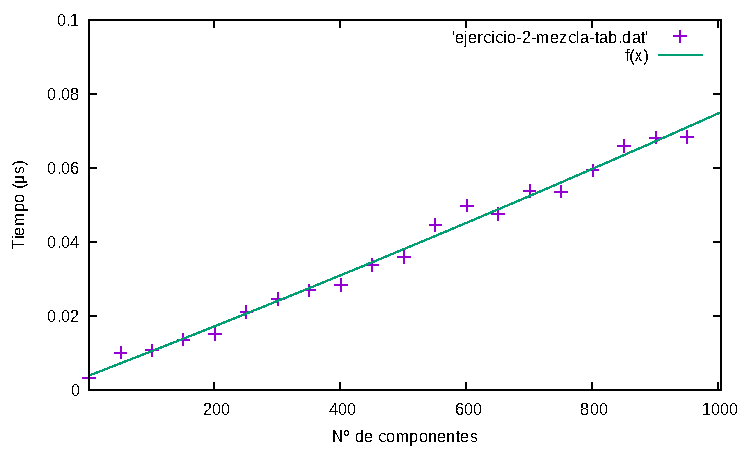
\includegraphics[scale=0.76]{img/ejercicio-2-obvio-graph.pdf}
    \caption{Gráfica de tiempos de ejecución para el caso obvio, 
    con f(x) y coeficiente de regresión especificada por \ref{eq:2a-ajuste}.}
    \label{fig:2a-obvio-graph}
\end{figure}
    \newpage

    \section{Conclusión}
    En conclusión, podemos observar que aunque el algoritmo greedy es muy eficiente, no siempre se trata del algoritmo óptimo para la resolución de un problema. 
En el primer ejercicio pudimos observar y demostrar que el algoritmo greedy es el óptimo para la resolución de ambos apartados. Sin embargo, en el ejercicio 2
vimos cómo un algoritmo greedy como el que nos inventamos, suponía unos tiempos de ejecución muy altos en comparación con los demás, lo que demuestra que no siempre
se trata del óptimo, puesto que hay algoritmos mejores.
Además nos hemos dado cuenta que existen distintos algoritmos greedy a la hora de enfocar un determinado problema y que no todos tienen por qué tener la misma eficiencia,
de hecho varía para distintas formas de atajar el problema. 

    \begin{thebibliography}{0}
        \bibitem{Verdegay2017} Verdegay Galdeano. (2017). Lecciones de Algorítmica / José Luis Verdegay. Técnica Avicam.
        \bibitem{Cormen2017} Cormen. (2017). Introduction to algorithms / Thomas H. Cormen... [et al.] (3rd ed.). PHI Learning.
        \bibitem{Garrido2018} Garrido Carrillo. (2018). Estructuras de datos avanzadas: con soluciones en C++ / A. Garrido. Universidad de Granada.  
    \end{thebibliography}
\end{document}